%!TEX root = ../thesis.tex
\define{\chapterpath}{appendix}
\define{\imgpath}{appendix/img}

%%
\chapter{Appendix}
\label{appendix}

%%%%%%%%%%%%%%%%%%%%%%%%%%%%%%%%%%%%%%%%%%%%%%
%%%%%%%%%%%%%%%%%%%%%%%%%%%%%%%%%%%%%%%%%%%%%%
%%%%%%%%%%%%%%%%%%%%%%%%%%%%%%%%%%%%%%%%%%%%%%
%%%%%%%%%%%%%%%%%%%%%%%%%%%%%%%%%%%%%%%%%%%%%%
%%%%%%%%%%%%%%%%%%%%%%%%%%%%%%%%%%%%%%%%%%%%%%
\section{Additional visuals of uncertainty}
\label{appendix:uncertaintymeaning}

This section present the illustration of the planning method relying on sampling teaching signal and  asking every hypothesis if each of those signals are expected or not for the given state-action pair. 

We present the case where the models between hypothesis are identical. As depicted in Figure~\ref{fig:uncertaintymeaningupdownexpectedright}, when selecting action down in state 3 and if the user sends a signal in the right part of the feature space, both hypothesis agree that this particular signal is unexpected given this state-action pair. Hypothesis 1 expects a signal of meaning ``incorrect'', and the teacher signal is classified as being of class ``correct''. Hypothesis 2 expects a signal of meaning ``incorrect'' and the teacher signal is classified as being of class ``correct''. Therefore receiving this particular signal after taking action down in state 3 has low uncertainty.

\begin{figure}[!htbp]
  \centering
  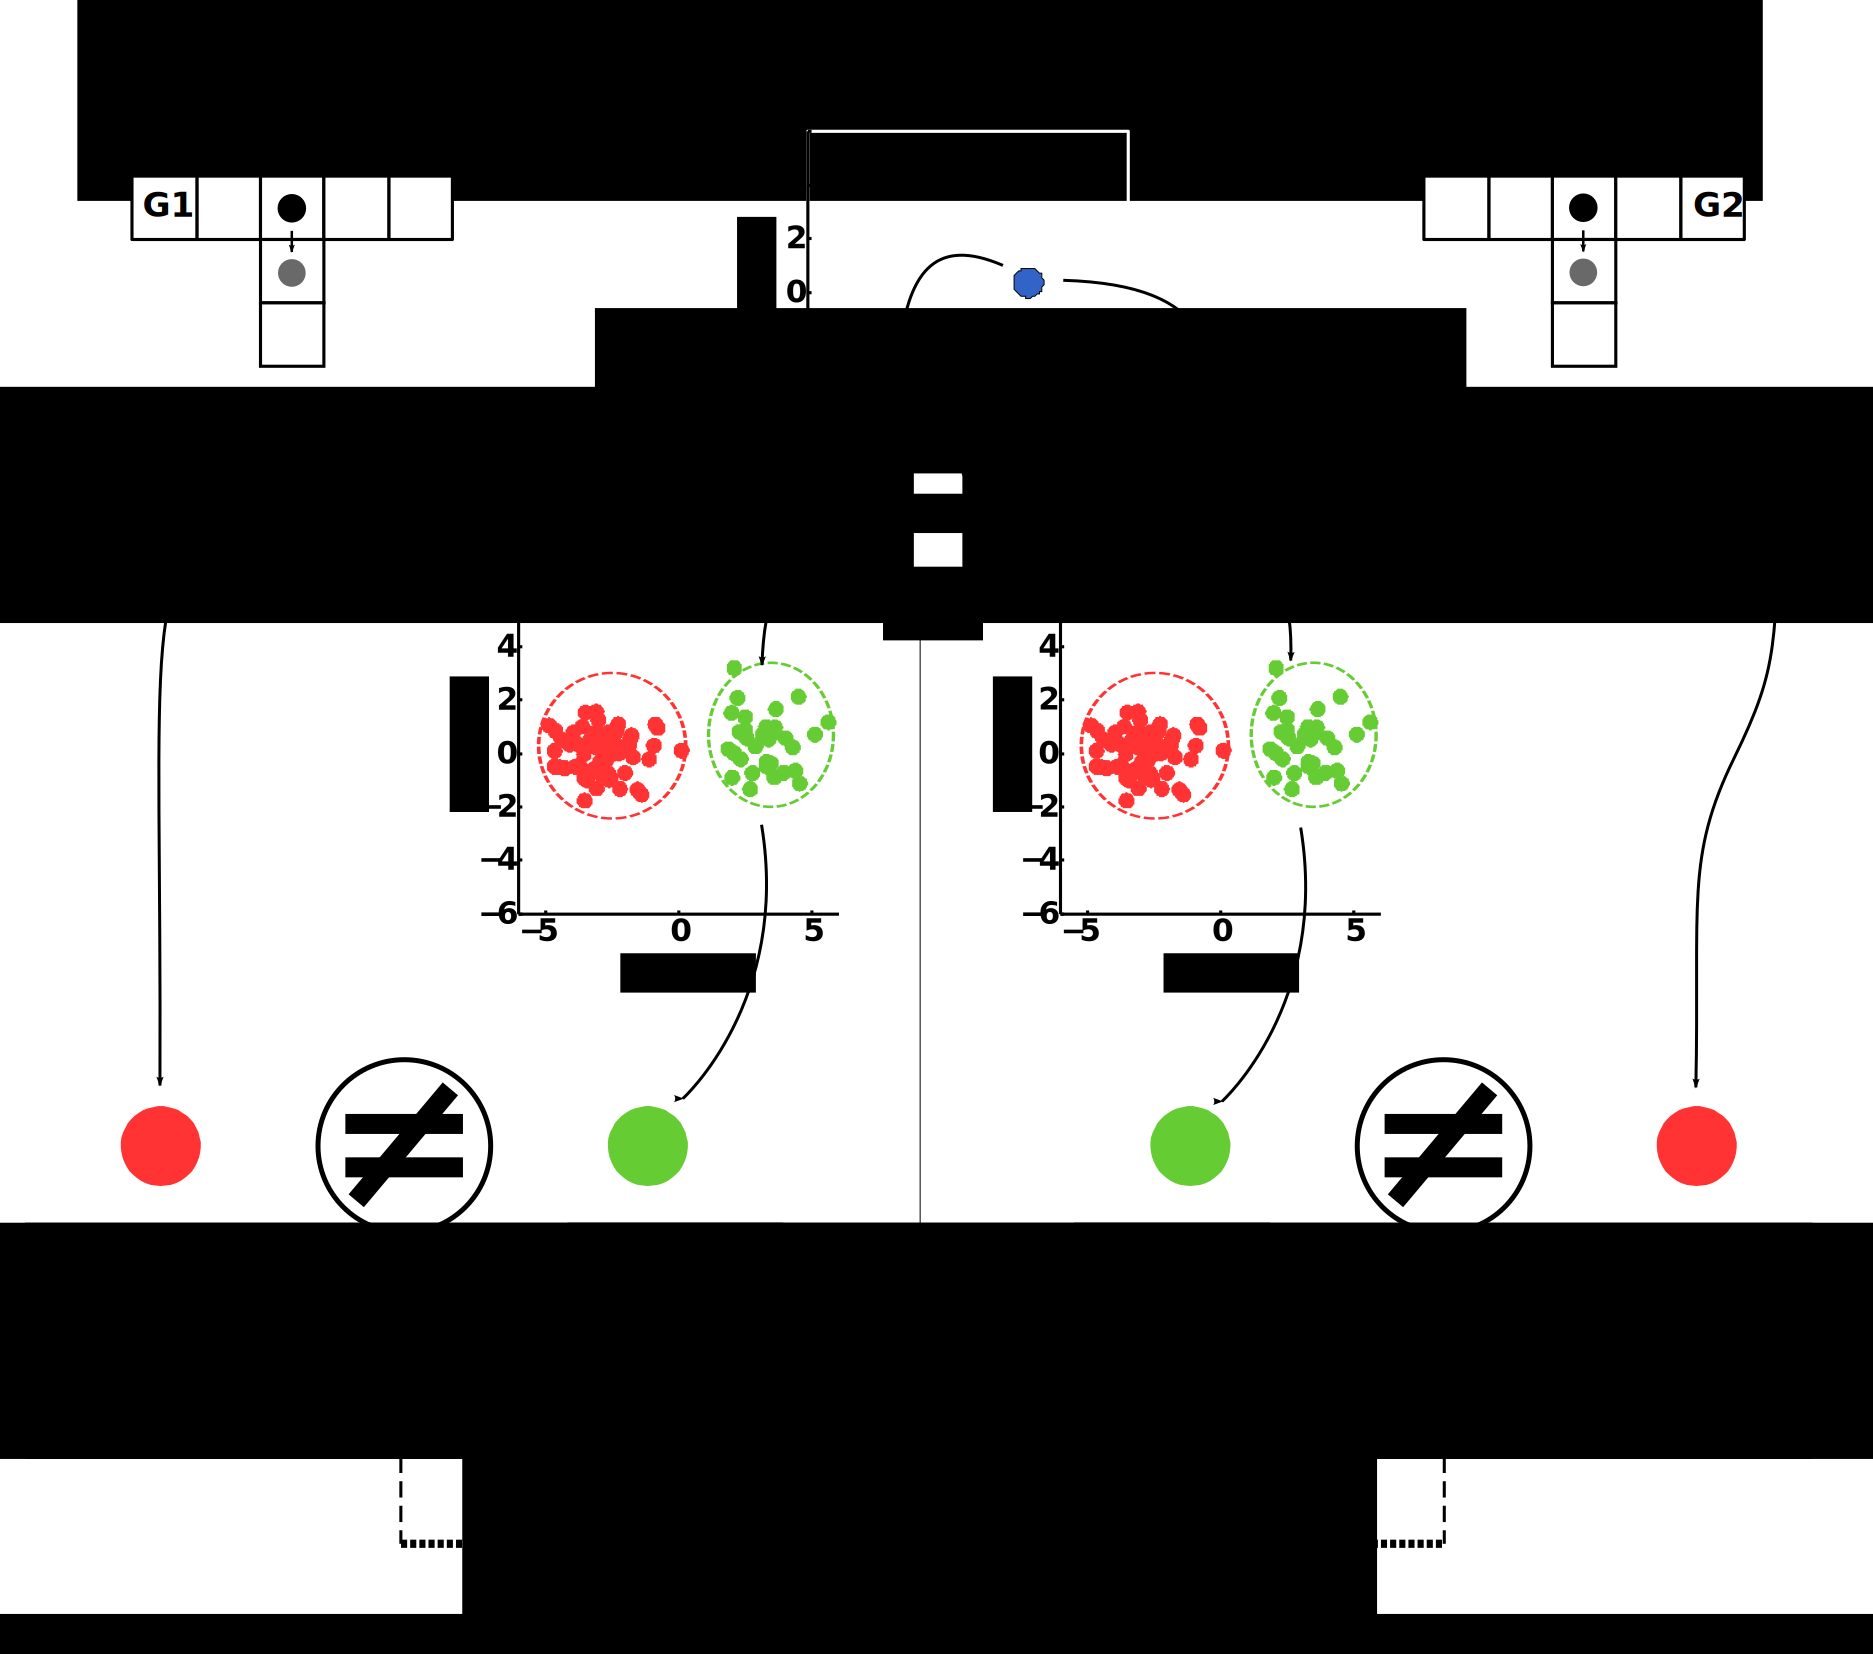
\includegraphics[width=\threeplanningwidth\columnwidth]{\visualspdf/planning/planning_up_down_expected_unmatched.pdf}
  \caption{Matching between expected labels and the prediction of a teaching signal sample on the right side of the feature space for the two hypothesis if the agent performs action down in state 3 and the two hypothesis currently have a symmetric interpretation of signals from Figure~\ref{fig:planningupdown}. Both hypothesis agree that the label associated to a signal on the right side of the feature space does not match with the label predicted given the frame and the state-action pair considered. Therefore there is no uncertainty associated to this state-action pair and the agent should not select action down in order to disambiguate between hypothesis.}
  \label{fig:uncertaintymeaningupdownexpectedright}
\end{figure}

This same process can be executed for any teaching signal. For example, as depicted in Figure~\ref{fig:uncertaintymeaningupdownexpectedleft}, considering a teaching signal on the left side of the feature space, if the agent performs action down in state 3, both hypothesis agree that this particular signal is expected. Hypothesis 1 expects a signal of meaning ``incorrect'', and the teacher signal is classified as being of class ``incorrect''. Hypothesis 2 expects a signal of meaning ``incorrect'' and the teacher signal is classified as being of class ``incorrect''. Therefore receiving this particular signal after taking action down in state 3 has low uncertainty.

\begin{figure}[!htbp]
  \centering
  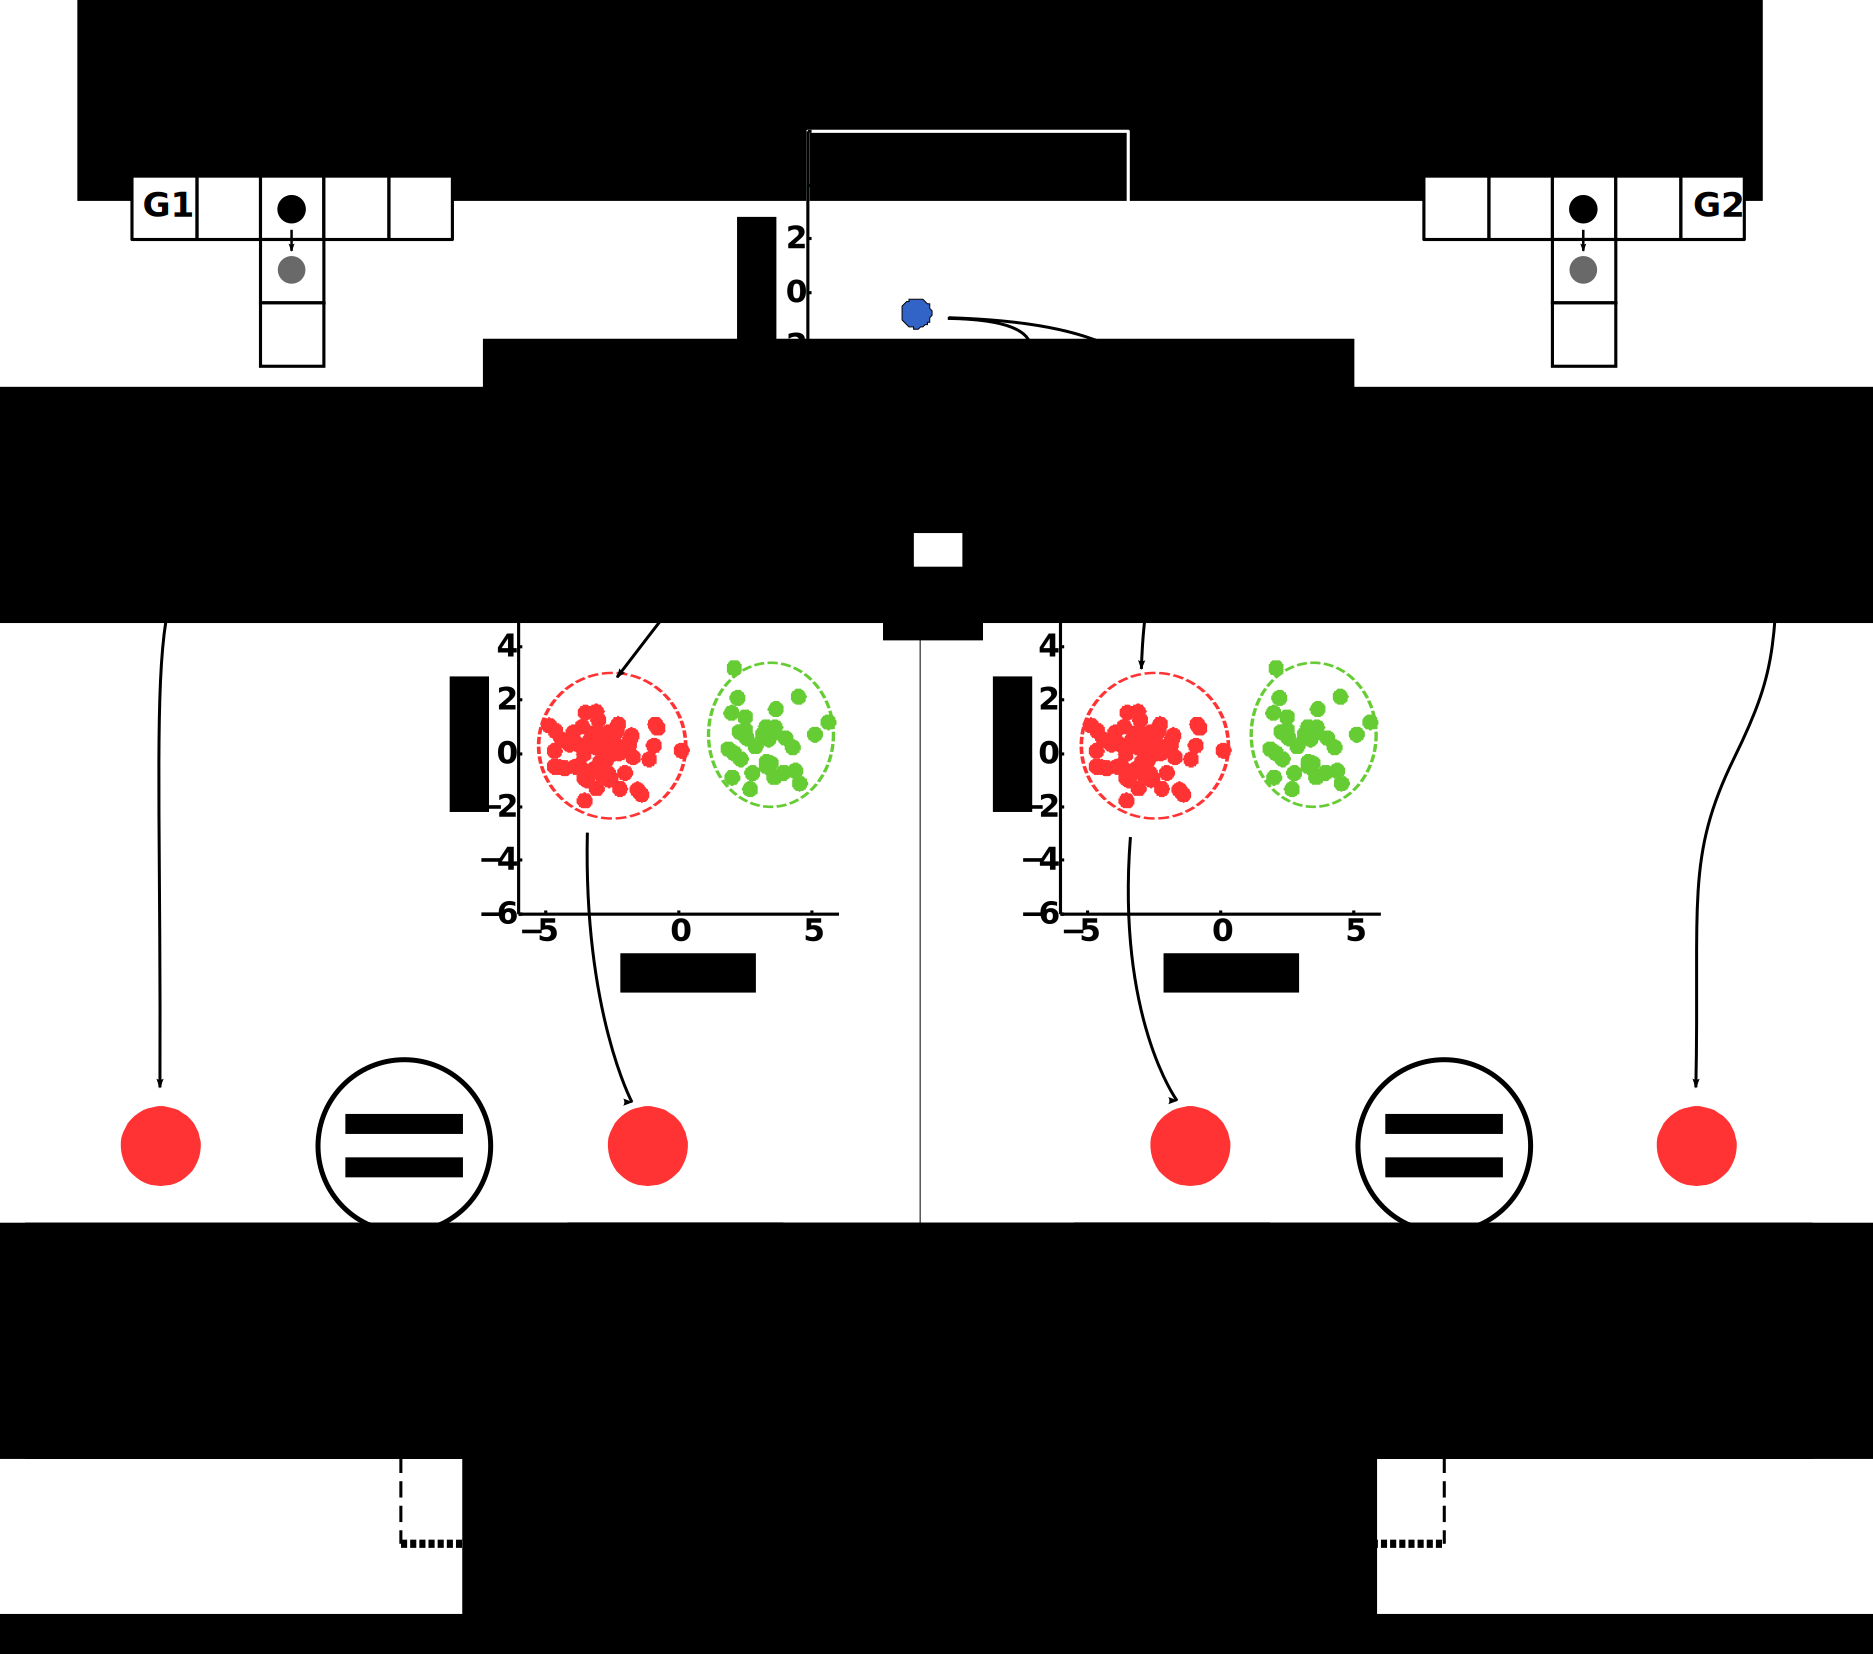
\includegraphics[width=\threeplanningwidth\columnwidth]{\visualspdf/planning/planning_up_down_expected_matched.pdf}
  \caption{Matching between expected labels and the prediction of a teaching signal sample on the left side of the feature space for the two hypothesis if the agent performs action down in state 3 and the two hypothesis currently have a symmetric interpretation of signals from Figure~\ref{fig:planningupdown}. Both hypothesis agree that the label associated to a signal on the left side of the feature space match with the label predicted given the frame and the state-action pair considered. Therefore there is no uncertainty associated to this state-action pair and the agent should not select action down in order to disambiguate between hypothesis.}
  \label{fig:uncertaintymeaningupdownexpectedleft}
\end{figure}

However for action left, the two hypothesis disagree on whether such signals are expected or not given the state-action pair considered. As depicted in Figure~\ref{fig:uncertaintymeaningupdownunexpectedright}, when selecting action left in state 3 and if the user sends a signal in the right part of the feature space, hypothesis 1 expects a signal of meaning ``correct'', and the teacher signal is classified as being of class ``correct''. And hypothesis 2 expects a signal of meaning ``incorrect'' and the teacher signal is classified as being of class ``correct''. Therefore receiving this particular signal after taking action down in state 3 is expected for hypothesis 1 but not expected for hypothesis 2, there is high uncertainty.

\begin{figure}[!htbp]
  \centering
  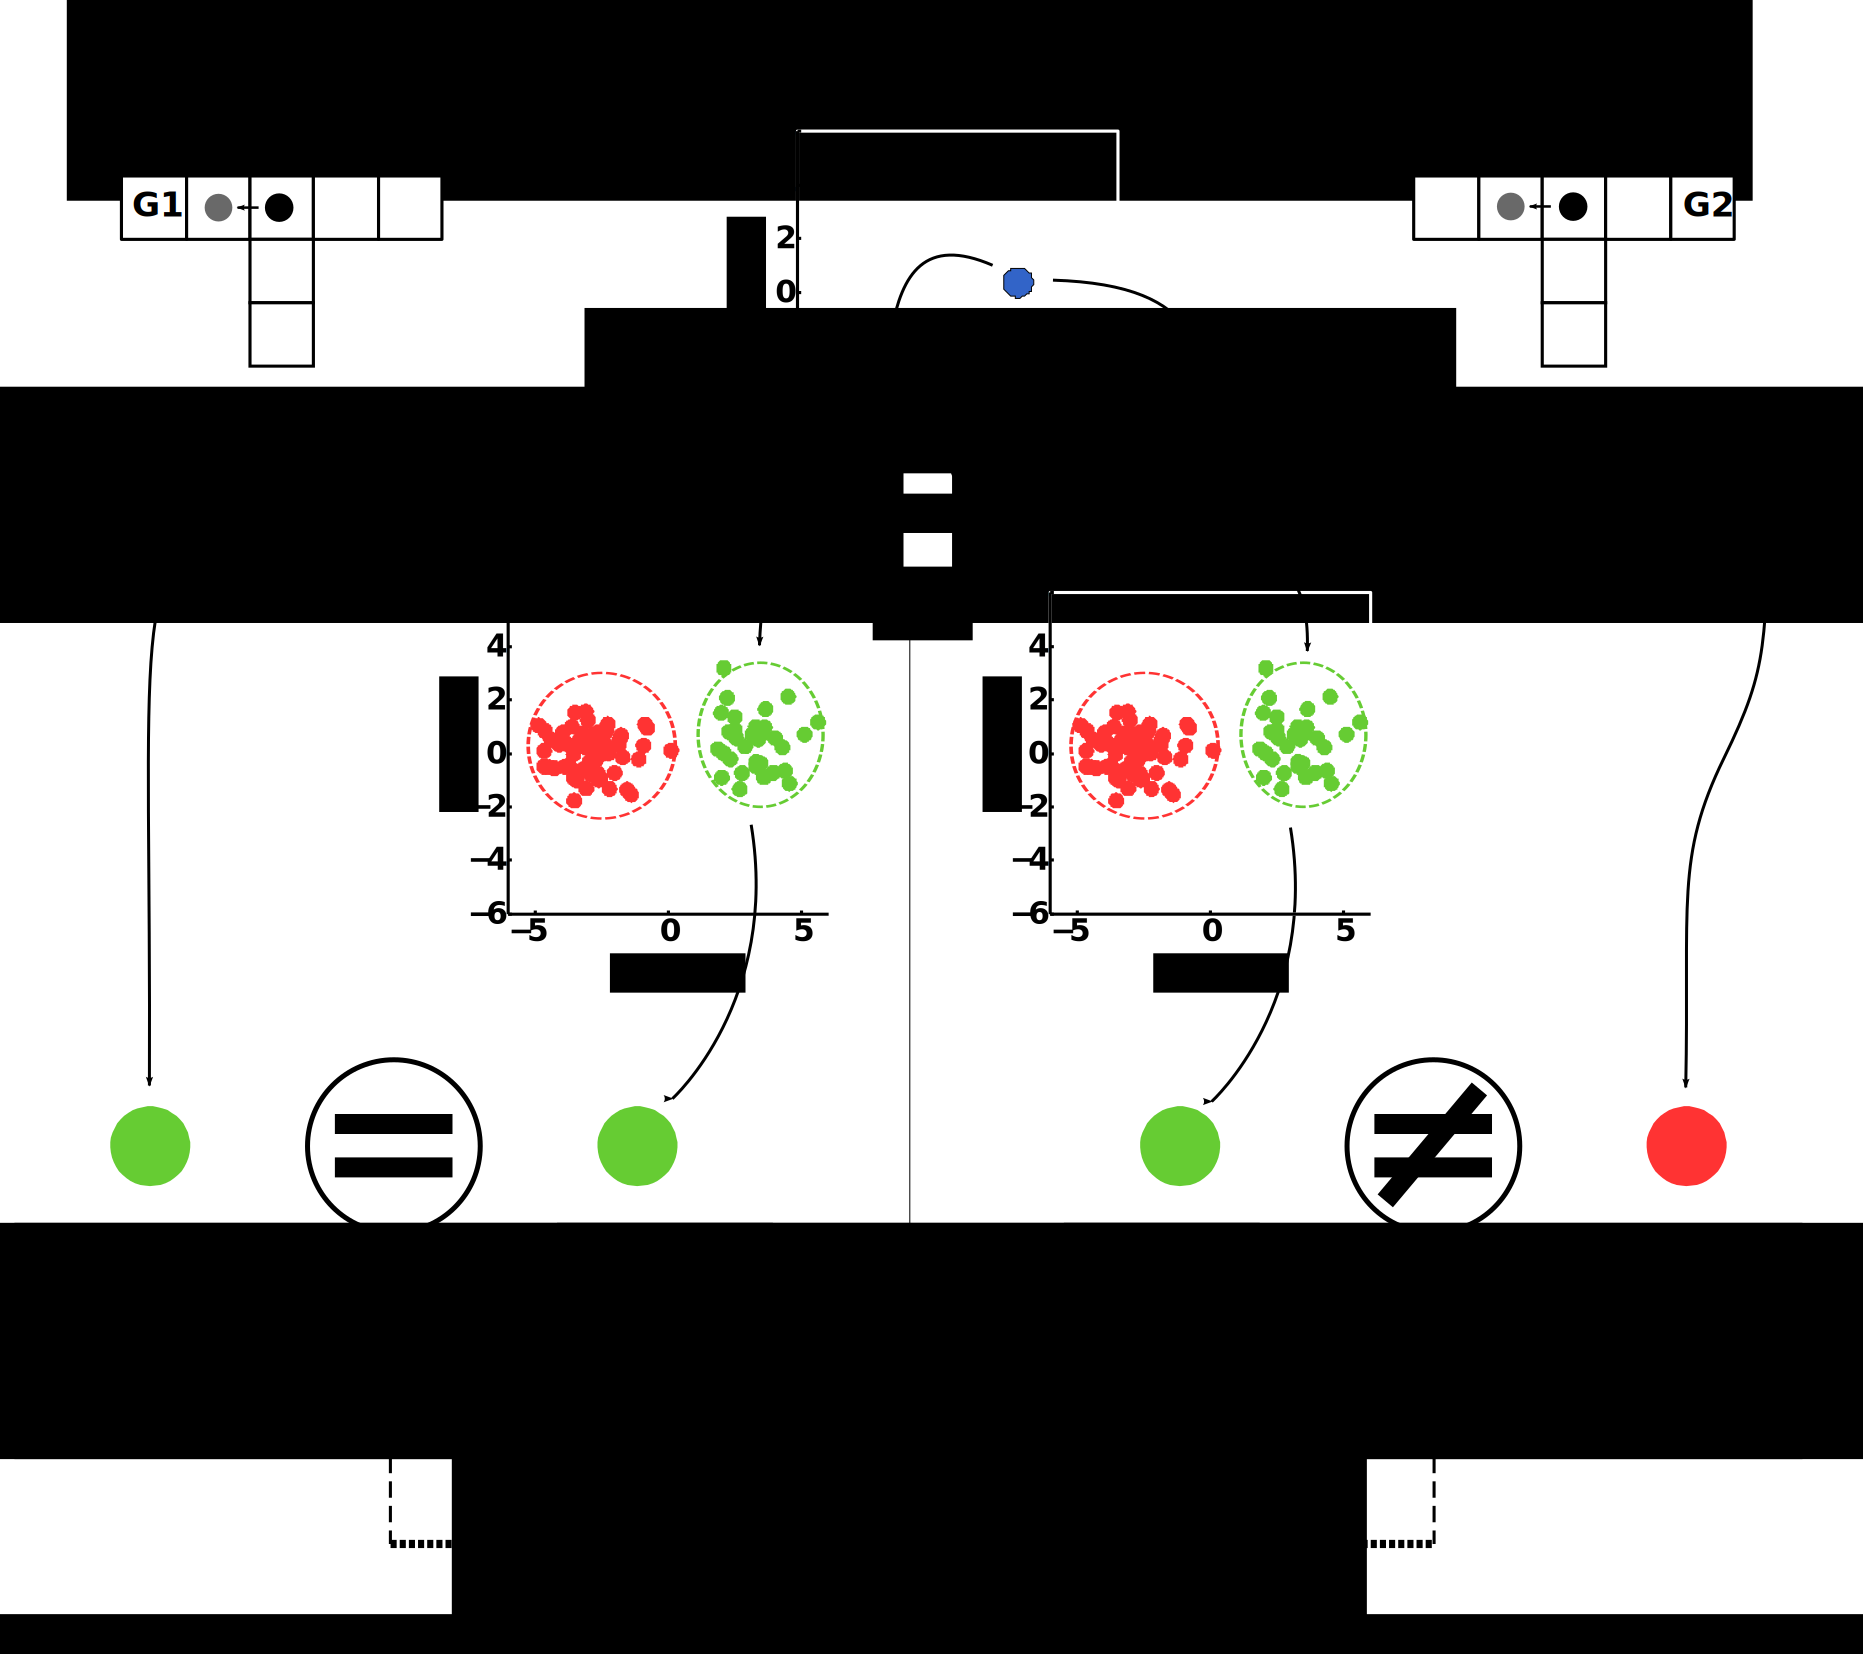
\includegraphics[width=\threeplanningwidth\columnwidth]{\visualspdf/planning/planning_up_down_unexpected_right_signal.pdf}
  \caption{Matching between expected labels and the prediction of a teaching signal sample on the right side of the feature space for the two hypothesis if the agent performs action left in state 3 and the two hypothesis currently have a symmetric interpretation of signals from Figure~\ref{fig:planningupdown}. Hypothesis 1 says a signal on the right side of the feature space means ``correct'' which was expected given the interaction frame, while hypothesis 2 expected a signal meaning ``incorrect'' but classify the signal as ``correct'' which was not expected. Therefore there is high uncertainty associated to this state-action pair and the agent should better perform action left in order to disambiguate between hypothesis.}
  \label{fig:uncertaintymeaningupdownunexpectedright}
\end{figure}

Similarly, as depicted in Figure~\ref{fig:uncertaintymeaningupdownunexpectedleft}, considering a teaching signal on the left side of the feature space, if the agent performs action left in state 3, hypothesis 1 expects a signal of meaning ``incorrect'', and the teacher signal is classified as being of class ``incorrect''. And hypothesis 2 expects a signal of meaning ``incorrect'' and the teacher signal is classified as being of class ``correct''. Therefore receiving this particular signal after taking action down in state 3 is not expected for hypothesis 1 but expected for hypothesis 2, there is high uncertainty.

\begin{figure}[!htbp]
  \centering
  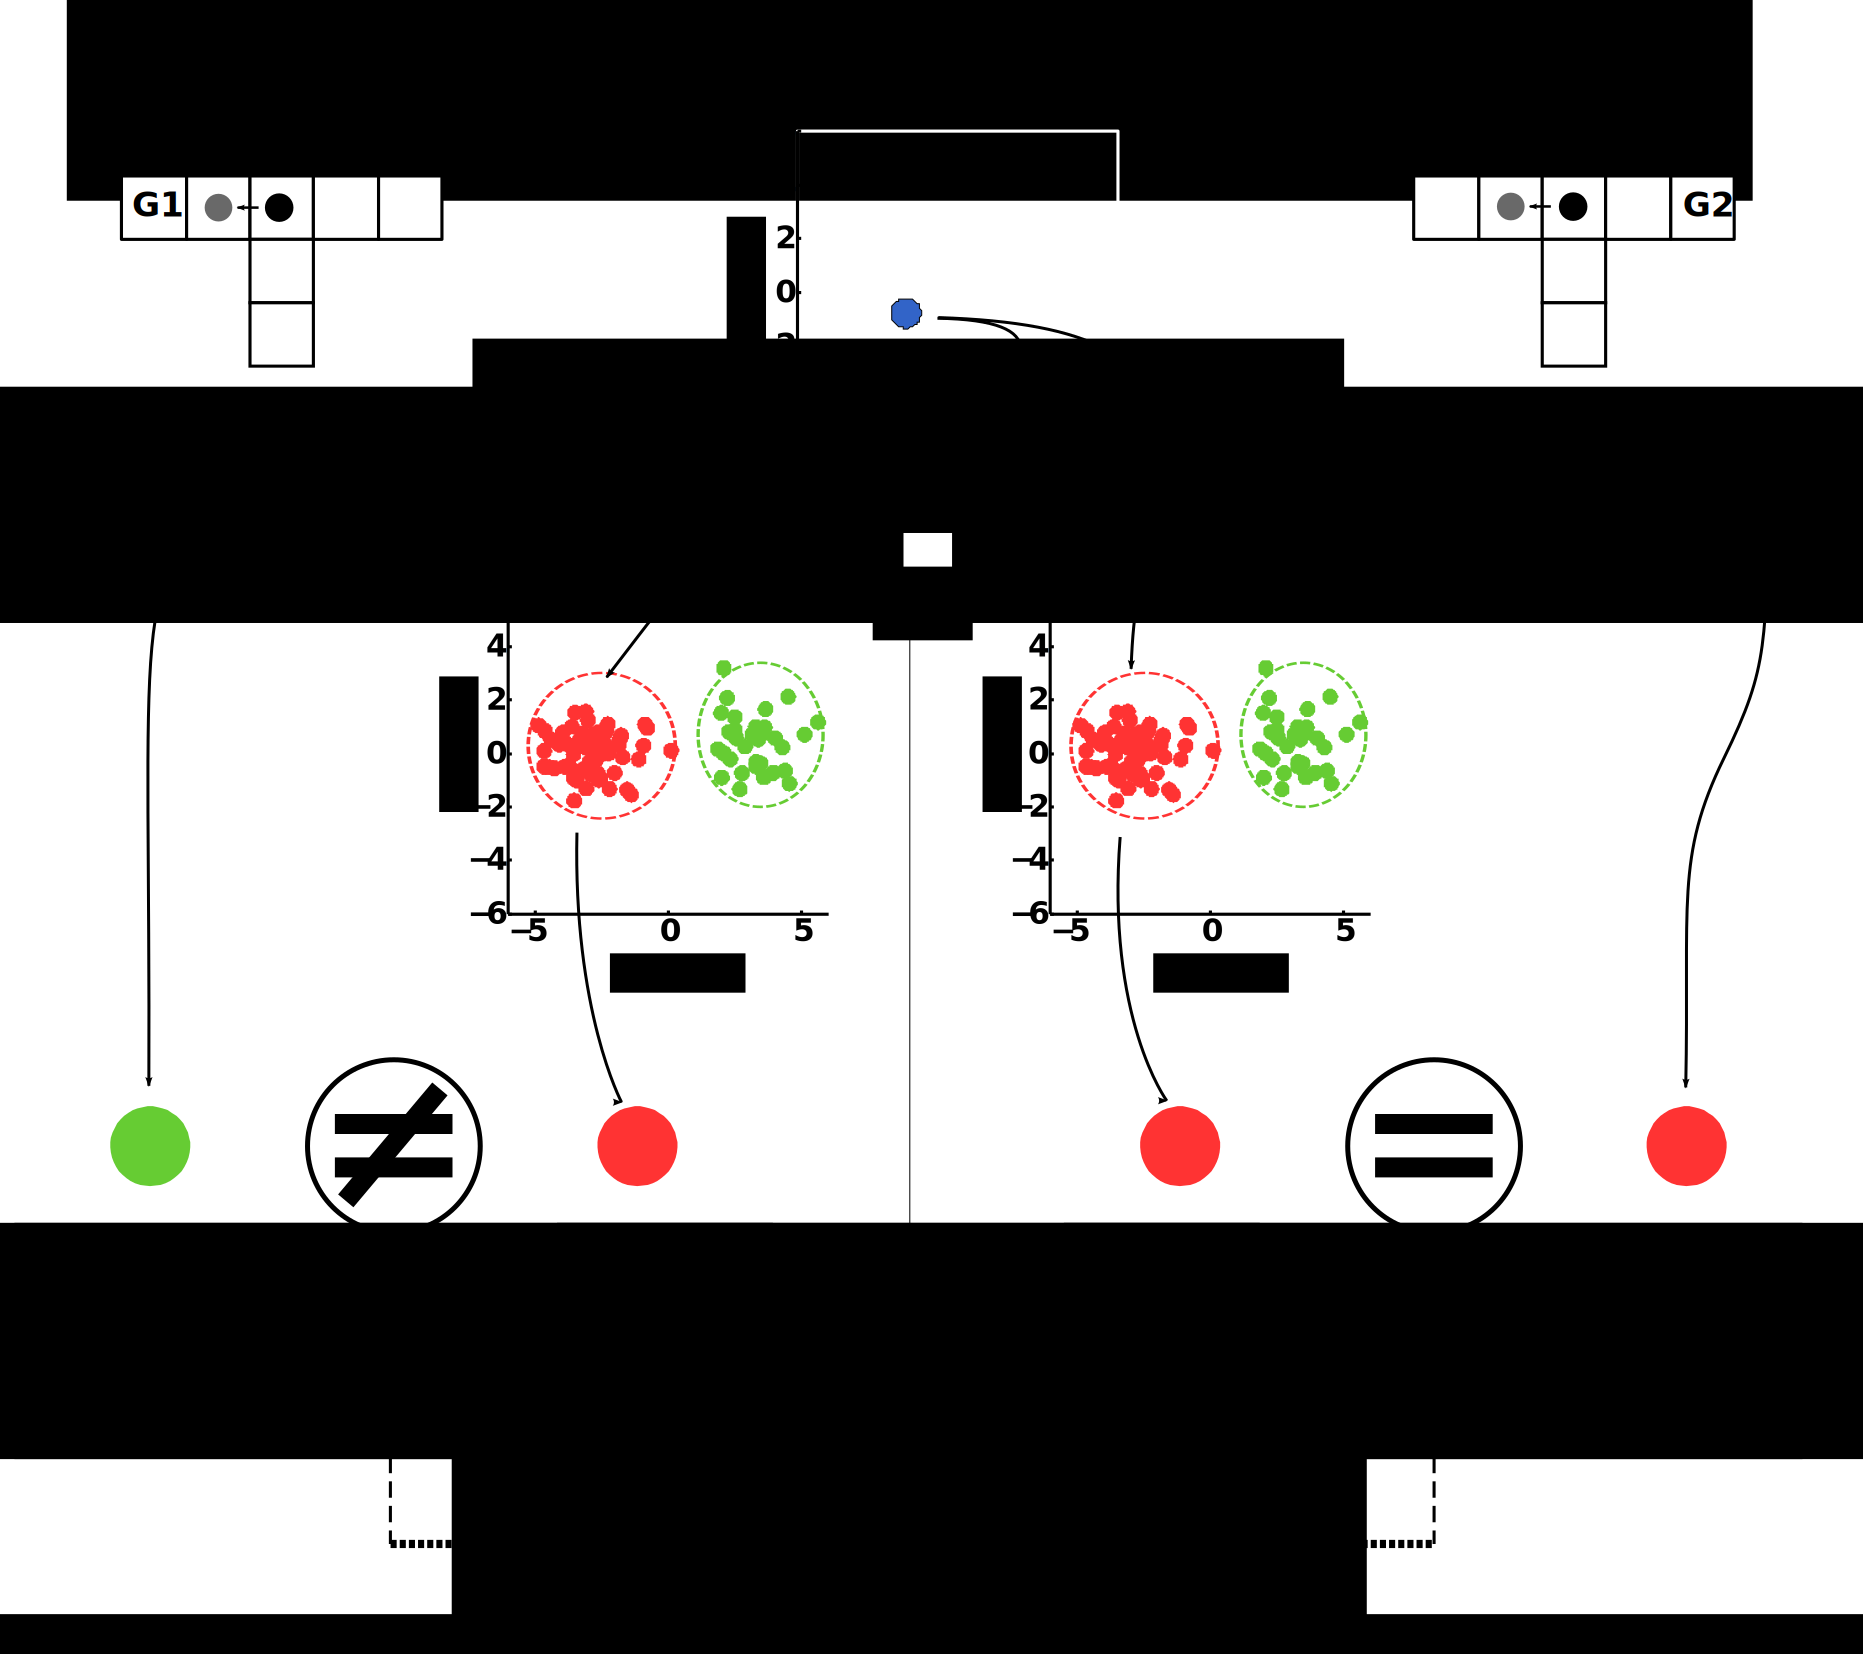
\includegraphics[width=\threeplanningwidth\columnwidth]{\visualspdf/planning/planning_up_down_unexpected_left_signal.pdf}
  \caption{Matching between expected labels and the prediction of a teaching signal sample on the left side of the feature space for the two hypothesis if the agent performs action left in state 3 and the two hypothesis currently have a symmetric interpretation of signals from Figure~\ref{fig:planningupdown}. Hypothesis 1 says a signal on the left side of the feature space means ``incorrect'' which was not expected given the interaction frame, while hypothesis 2 expected a signal meaning ``incorrect'' and classify the signal as ``incorrect'' which is what was expected. Therefore there is high uncertainty associated to this state-action pair and the agent should better perform action left in order to disambiguate between hypothesis.}
  \label{fig:uncertaintymeaningupdownunexpectedleft}
\end{figure}


%%%%%%%%%%%%%%%%%%%%%%%%%%%%%%%%%%%%%%%%%%%%%%
%%%%%%%%%%%%%%%%%%%%%%%%%%%%%%%%%%%%%%%%%%%%%%
%%%%%%%%%%%%%%%%%%%%%%%%%%%%%%%%%%%%%%%%%%%%%%
%%%%%%%%%%%%%%%%%%%%%%%%%%%%%%%%%%%%%%%%%%%%%%
%%%%%%%%%%%%%%%%%%%%%%%%%%%%%%%%%%%%%%%%%%%%%%
\section{Illustration of the gridworld scenario}
\label{appendix:gridworld}

In chapter~\ref{chapter:planning}, we consider a 5x5 grid world, where an agent can perform five different discrete actions: move up, down, left, right, or a ``no move'' action. The user goal is to teach the agent to reach one (unknown to the agent) of the 25 discrete positions which represent the set of possible tasks. We also consider the user is providing feedback on the agent action. We illustrate in Figure~\ref{fig:appendix:gridworldfeedback}, a smaller 3x3 grid world example and the results of the hypothetic labeling process. As the teacher is providing feedback with respect to hypothesis 1, the labeling process for hypothesis 1 is more coherent with the spacial organization of the data. We note that hypothesis 9 has symmetric properties with hypothesis 1 but the use of the ``no move'' allow to break that symmetry.

\begin{figure}[!htbp]
  \centering
  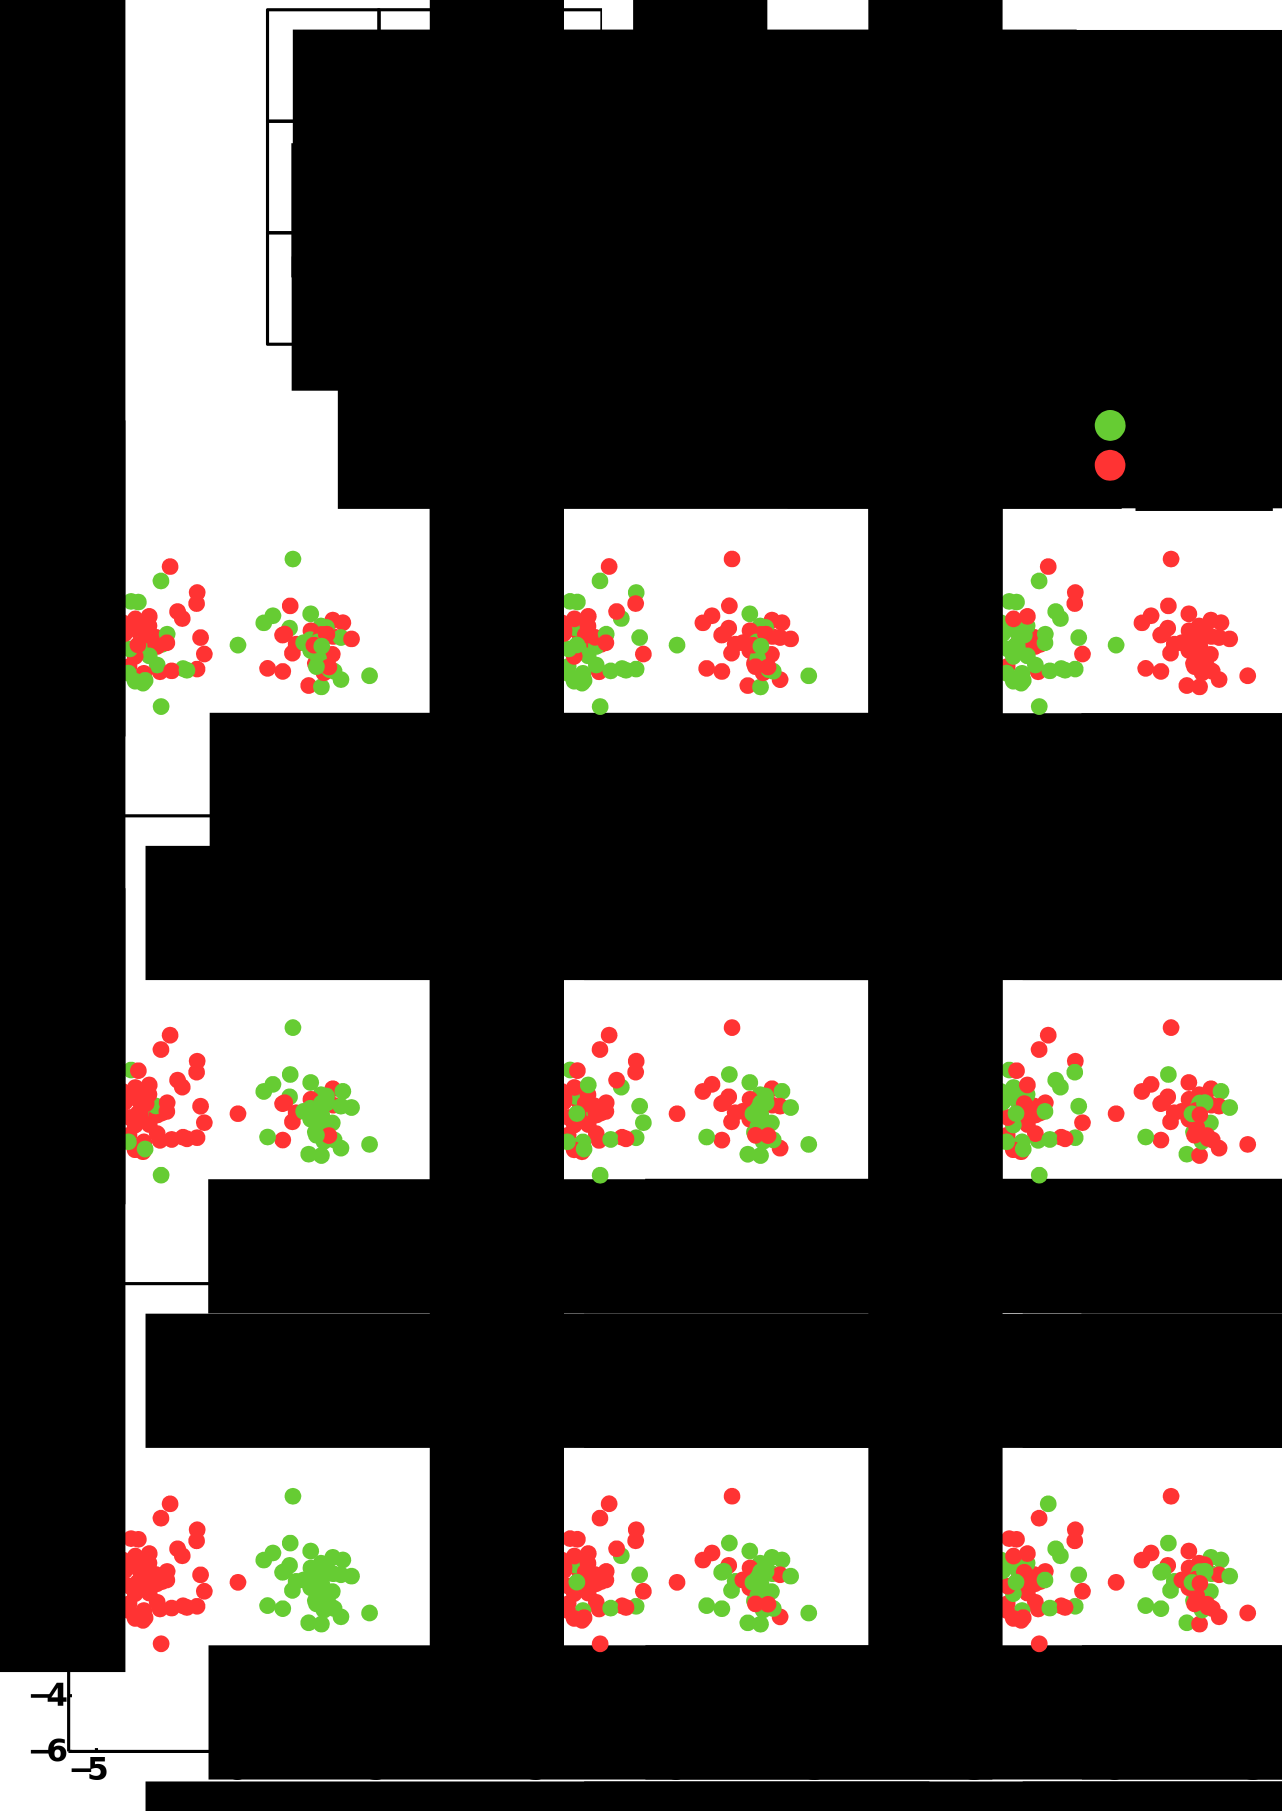
\includegraphics[width=\columnwidth]{\visualspdf/gridworld/gridworld_feedback.pdf}
  \caption{A schematic view of a 3x3 grid world scenario. There is nine possible hypothesis and the agent is acting randomly for this example. We show the results of the per hypothesis labeling process considering the feedback frame. The teacher is providing feedback with respect to hypothesis 1. The labeling process for hypothesis 1 is more coherent with the spacial organization of the data which indicates it is the one taught by the user. Hypothesis 9 has symmetric properties with hypothesis 1 but the use of the ``no move'' allow to break that symmetry.}
  \label{fig:appendix:gridworldfeedback}
\end{figure}

%%%%%%%%%%%%%%%%%%%%%%%%%%%%%%%%%%%%%%%%%%%%%%
%%%%%%%%%%%%%%%%%%%%%%%%%%%%%%%%%%%%%%%%%%%%%%
%%%%%%%%%%%%%%%%%%%%%%%%%%%%%%%%%%%%%%%%%%%%%%
%%%%%%%%%%%%%%%%%%%%%%%%%%%%%%%%%%%%%%%%%%%%%%
%%%%%%%%%%%%%%%%%%%%%%%%%%%%%%%%%%%%%%%%%%%%%%
\section{Details of the likelihood function factorization}
\label{appendix:proof}

We remind the likelihood equation:
%
\begin{eqnarray}
\L(\xi_t) &=& \prod_{i = 1,\ldots,M} p(l^c_i = l^f_i | D_M, \xi_t) \nonumber \\ 
&=& \prod_{i = 1,\ldots,M} \sum_{k = 1, \ldots, L} p(l^c_i = l_k | e_i, \theta_M) p(l^f_i = l_k | s_i, a_i, \xi_t) \nonumber
\end{eqnarray}
%
where $p(l^c_i = l_k | e_i, \theta_M)$ is the classification of the signal $e_i$ from our classification model $\theta_M$, and $p(l^f_i = l_k | s_i, a_i, \xi_t)$ is the expected label given by the frame.

Following our simple symbolic example of chapter~\ref{chapter:limitations:proof}, the expected labels are either ``correct'' or ``incorrect'' and, as the user makes not mistake, the probabilities are either 0 or 1. We denote $[1,0]_{s_i,a_i,\xi_t}$ the vector of probability which associate a probability of 1 for the meaning ``correct'' (i.e. $p(l^f_i = ``correct" | s_i, a_i, \xi_t) = 1$ ) and of 0 for the meaning ``incorrect'' (i.e. $p(l^f_i = ``incorrect" | s_i, a_i, \xi_t) = 0$ ). Respectively for the non-optimal state-action pairs, this vector becomes $[0,1]_{s_i,a_i,\xi_t}$.

Similarly, given our development of chapter~\ref{chapter:limitations:proof}, and assuming the agent visited all state-action pairs once, if the user uses the blue button to mean ``correct'', then the blue signal model will be $[\Upsilon_{\xi_t},1-\Upsilon_{\xi_t}]_{B,\xi_t}$. Which implies the orange button mapping is $[1-\Upsilon_{\xi_t},\Upsilon_{\xi_t}]_{O,\xi_t}$. Respectively, if the user uses the blue button to mean ``incorrect'', then the blue signal model will be $[1-\Upsilon_{\xi_t},\Upsilon_{\xi_t}]_{B,\xi_t}$. Which implies the orange button mapping is $[\Upsilon_{\xi_t},1-\Upsilon_{\xi_t}]_{O,\xi_t}$.  Where $\Upsilon_{\xi_t} = \frac{nSA - diff(\pi_t, \hat{\pi})}{nSA}$ denote the ratio of optimal state-action pairs of $\xi_t$ that are the same as for the true task $\hat{\xi}$.

Using this notation, we can write the likelihood equation as a product of vector's products. Where for example, $\sum_{k = 1, \ldots, L} p(l^c_i = l_k | e_i, \theta_M) p(l^f_i = l_k | s_i, a_i, \xi_t)$ can be written as $[\Upsilon_{\xi_t},1-\Upsilon_{\xi_t}]_{B,\xi_t}.[1,0]_{s_i,a_i,\xi_t}^T$ for those cases where the user pressed the blue button (i.e. $e_i = B$) after an optimal state-action pair (i.e. the expected meanings is ``correct'', i.e. $[1,0]_{s_i,a_i,\xi_t}$), and given that the blue button was the one used by the teacher to mean ``correct'', resulting in $[\Upsilon_{\xi_t},1-\Upsilon_{\xi_t}]_{B,\xi_t}$ as the button to meaning model.

Let's now list all the possible cases. We can split the state-action pairs in half, the one that are optimal according to the teacher intended task $\hat{\xi}$ (there is $\frac{nSA}{2}$ of them) and the one that are non-optimal according to the teacher intended task $\hat{\xi}$ (there is $\frac{nSA}{2}$ of them). For the state-action pairs that are optimal, the user will press the button he uses to mean ``correct'' (i.e. the blue or the orange one), respectively for the non-optimal, he will press the other button (i.e. the orange or the blue one).

But the agent evaluates those button presses with respect to the task hypothesis currently considered $\xi_t$, which might not be the one the teacher as in mind. Therefore, only a fraction of the time the button presses match with what is expected by the task considered $\xi_t$. This number can be exactly identified as $\frac{nSA}{2}.\Upsilon_{\xi_t}$. Therefore for $\frac{nSA}{2}.\Upsilon_{\xi_t}$ state-action pairs, the ``correct'' button was pressed for the ``correct'' meaning. For one state-action pair, this represent an update of the likelihood function by $[\Upsilon_{\xi_t},1-\Upsilon_{\xi_t}].[1,0]^T$, which is simply $\Upsilon_{\xi_t}$. As there is $\frac{nSA}{2}.\Upsilon_{\xi_t}$ similar situations the update is $\Upsilon_{\xi_t}^{\frac{nSA}{2}.\Upsilon_{\xi_t}}$.

Similarly there is $\frac{nSA}{2}.(1-\Upsilon_{\xi_t})$, where the ``incorrect'' button was pressed for the ``correct'' meaning. Which represent an update of $[\Upsilon_{\xi_t},1-\Upsilon_{\xi_t}].[0,1]^T$, which is simply $1-\Upsilon_{\xi_t}$. As there is $\frac{nSA}{2}.(1-\Upsilon_{\xi_t})$ similar situations the update is $(1-\Upsilon_{\xi_t})^{\frac{nSA}{2}.(1-\Upsilon_{\xi_t})}$.

And as the situation is symmetric for the non-optimal state-action pair of the teacher intended task $\hat{\xi}$, the likelihood equation can be rewritten as:

\begin{eqnarray}
\L(\xi_t) &=& \Upsilon_{\xi_t}^{\frac{nSA}{2}.\Upsilon_{\xi_t}} \times (1-\Upsilon_{\xi_t})^{\frac{nSA}{2}.(1-\Upsilon_{\xi_t})} \times \Upsilon_{\xi_t}^{\frac{nSA}{2}.\Upsilon_{\xi_t}} \times (1-\Upsilon_{\xi_t})^{\frac{nSA}{2}.(1-\Upsilon_{\xi_t})} \nonumber \\
&=& \Upsilon_{\xi_t}^{nSA.\Upsilon_{\xi_t}} \times (1-\Upsilon_{\xi_t})^{nSA.(1-\Upsilon_{\xi_t})} \nonumber
\end{eqnarray}

Note that this equation is the same whatever the button chosen by the user to mean ``correct''.








